\documentclass[a4paper,12pt]{article}
%\usepackage{fullpage}
%\usepackage{a4wide}
\usepackage[utf8]{inputenc}
\usepackage[danish, english]{babel}

% Nice looking font
%\usepackage{palatino}

% Minitoc - mini table of contents
\usepackage{minitoc}

% In order to highlight code
\usepackage[pdftex]{color}
\usepackage{listings}

% For graphics support
\usepackage{epsfig}
\usepackage{graphicx}
\usepackage{subfigure}

% Math support
\usepackage{amsmath}
\usepackage{amssymb}

% In order to include pdf
\usepackage{pdfpages}

% Graf support
\usepackage{tkz-graph}

% Pdf section support
\usepackage{hyperref}
\hypersetup{
    bookmarks=true,         % show bookmarks bar?
    unicode=false,          % non-Latin characters in Acrobat's bookmarks
    pdftoolbar=false,       % show Acrobat's toolbar?
    pdfmenubar=false,       % show Acrobat's menu?
    pdffitwindow=true,      % page fit to window when opened
    pdftitle={OCamlCSP. A concurrency library for Ocaml}, % title
    pdfauthor={Joakim Ahnfelt-Rønne - 1986/03/14 - joakim.ahnfelt@gmail.com,
        Ramón Salvador Soto Mathiesen - 1979/05/15 - ramon@diku.dk and
        Advisor: Andrzej Filinski - andrzej@diku.dk}, % author
    pdfsubject={},   % subject of the document
    pdfnewwindow=true,      % links in new window
    pdfkeywords={keywords}, % list of keywords
    colorlinks=false,       % false: boxed links; true: colored links
    linkcolor=red,          % color of internal links
    citecolor=green,        % color of links to bibliography
    filecolor=magenta,      % color of file links
    urlcolor=cyan           % color of external links
}

% Macros
\newcommand{\missing}[1]{
  \begin{tabular}{|p{11cm}|}
    \hline
    \emph{Missing:} {\scriptsize (things that need to be written or considered)} \\
    \hline
    #1
    \hline
  \end{tabular}
}

\newcommand{\runtest}[1]{
  \footnotesize
  \framebox[14.5cm][l]{#1}
  \normalsize
}

\newcommand{\includecode}[2]{
  \definecolor{stringcolor}{rgb}{0.50,0.00,0.50}      %
  \definecolor{commentcolor}{rgb}{0.00,0.50,0.00}     %
  \definecolor{keywordcolor}{rgb}{0.00,0.00,1.00}     %
  \definecolor{idcolor}{rgb}{0.00,0.00,0.00}          %
  \lstset{language=ML,basicstyle=\ttfamily,keywordstyle=\color{keywordcolor},
    commentstyle={\color{commentcolor}\itshape},
    stringstyle={\color{stringcolor}},
    identifierstyle=\color{idcolor},numbers=left,
    xleftmargin=2em,% framerule=0.8pt,
    stepnumber=1,frame=tlrb,showstringspaces=false,
    firstnumber=1,numberstyle=\ttfamily, breaklines}

  \normalsize
  #1:
  \scriptsize
  \lstinputlisting{#2}
  \normalsize
}

\newcommand{\includeoutput}[2]{
\definecolor{allblackcolor}{rgb}{0.00,0.00,0.00}      %
\lstset{basicstyle=\ttfamily,keywordstyle=\color{allblackcolor},
        commentstyle={\color{allblackcolor}\itshape},
        stringstyle={\color{allblackcolor}},
        identifierstyle=\color{allblackcolor},numbers=left,
        xleftmargin=2em,% framerule=0.8pt,
        stepnumber=0,frame=tlrb,showstringspaces=false,
        firstnumber=1,numberstyle=\ttfamily, breaklines}

  \normalsize
  #1:
  \scriptsize
  \lstinputlisting{#2}
  \normalsize
}

% Opening
\title{OCamlCSP - a concurrency library for Ocaml}
\author{Joakim Ahnfelt-Rønne - 1986/03/14 - joakim.ahnfelt@gmail.com \and 
        Ramón Salvador Soto Mathiesen - 1979/05/15 - ramon@diku.dk \and
        \\ Advisor: Andrzej Filinski - andrzej@diku.dk}
\date{31$^{st}$ July 2009}

\begin{document}

\maketitle

\newpage
\selectlanguage{english}
\begin{abstract}
% Grue: Højest 10 linjer: Hvad handler rapporten om? Hvilke resultater er
% opnået?
We present a concurrent library in a functional language designed and
implemented after the abstracts of CSP\cite{hoare}. The library can't offer true
parallelism due to the limitation of the chossen programming language but we can
offer overlapping I/O operations.
\\ \\
We provide some examples on how to implement components with the concurrent
library.
\\ \\
TODO: some more here ...
\end{abstract}

\newpage
\setcounter{tocdepth}{2}
\setcounter{secttocdepth}{3}
\dosecttoc \tableofcontents
\newpage

% Line breaks between paragraphs instead of indentation
\parindent=0pt
\parskip=8pt plus 2pt minus 4pt

\section{Introduction}
When we took the course Extreme Multiprogramming 2009 at the Department of
Computer Science, Copenhagen University, we missed a CSP\cite{hoare} library for
a functional programming language. All the presented libraries were for
imperative languages. We missed a library that was based on ML or functional
programming in general.

We have designed and implemented the abstracts of CSP in a functional
language\cite{ocaml}. In the chossen programming language, Ocaml, we found out
that there already was a concurrent library, {\it Event}, but this was inspired
on {\it ConcurrentML} and not on CSP as ours. Whenever we didn't find a
theoretical guidance from \cite{hoare} on how to implement ``TODO:something'',
for example shutting correctly down a network, we used the other CSP libraries,
\cite{pycsp}, \cite{jcsp} and \cite{cppcsp2}, as inspiration (poison).

One of our goals was to offer true parallelism, run several processors
over several CPUs or cores, but the library cannot offer this because of the
limitations of Ocaml, see {\it appendix \ref{appendixSysthreads}}. Based on
Xavier Leroys $[$ Cam-list $]$ answer we can see that the goals for threads in a
Ocaml context is to offer:
\begin{itemize}
 \item {\it Overlapping I/O and computation}.
 \item {\it Supporting the "coroutine" programming style}.
\end{itemize}
but not {\it Parallelism on shared-memory multiprocessors}. Even though we can't
offer parallelism over several multiprocessors or kernels we can still offer
concurrency over a single processor and {\it Overlapping I/O and computation}.
Thanks to this we have been able to implement a Webproxy, see section
\ref{examples} for more information, with non-blocking I/O.

Besides the implementation of the Webproxy, we also implemented a CSP
Library ({\it Legoland\cite{vinterpycsp}}), with these components we are able to
create simple networks as the one that gives us Fibonacci numbers, see section
\ref{examples}. But just to show how simple it is to write a CSP network with
our library we show the following example where we print even numbers in
$\mathbb{N}$:
\newpage
\begin{verbatim}
let rec counter n o () =
  Csp.write o n; counter (n+1) o ()

let rec double i o () =
  let x = Csp.read i in
  Csp.write o (x*2); double i o ()

let rec print i () =
  print_endline(string_of_int (Csp.read i)); print i ()

let even_numbers o () =
  let c = Csp.new_channel () in
    Csp.parallel [
      counter 1 c;
      double c o;
    ]

let _ =
  let c = Csp.new_channel () in
    Csp.parallel [
      even_numbers c;
      print c
    ]
\end{verbatim}
We have a counter component, which sends a number over a channel and another
component which recieves a number from a input channel and sends the
double of the value through an output channel. If we combine those two
components together by running in parallel and we give the counter $1$ as
initial parameter we have a new component that will gives us the even numbers in
$\mathbb{N}$.

The resulting API source code, CSP utility and component library, and
documentation can be seen in the appendix \ref{appendixSrc} and \ref{appendixDoc}.
A online version is also avaliable at:

\begin{center}
http://github.com/Ahnfelt/mlcsp/
\end{center}


\section{API design}
\label{apidesign}

The CSP theory is concerned with processes that communicate solely by synchronous 
events. Synchronous channels are built on top of the basic abstraction, and this is
what most implementations (including \cite{occam}, \cite{cppcsp2}, \cite{jcsp} and 
\cite{pycsp}) provide for communication. 
Additionally, it is possible to wait for communication from multiple sources at once.

For each construct, we are going to look at how it's done in CSP and in the 
existing CSP libraries, how we would like to write it in OCaml, and what the 
semantics should be. We will use the explicit module prefix \verb|Csp.| in front
of any functions that come from our API.

We have tried to mantain the API as small as possible. It's always easier to
learn an API which has a few methods instead of a well documented API as JCSP
but with a lot of classes and methods. We have moved everything out from the
library that was not strictly neccesary.

\subsection{Processes}
Processes can be run in parallel in CSP using the $\parallel$ operator:
\[P \parallel Q\]
The semantics of this is that the two processes $P$ and $Q$ are run in parallel. They
may communicate with each other. If put in front of another process in a sequence, all
processes running in parallel must finish before the next process can take any steps.

In PyCSP running two processes in parallel looks like this:
\begin{verbatim}
Parallel(P, Q)
\end{verbatim}
Where $P$ and $Q$ must be specified as $Process$ instances. There may be more processes
separated by commas. It runs the processes in parallel and returns when they have all 
stopped executing. Thes API for C++CSP2 and JCSP are similar. In all cases the
process objects only expose a \emph{run} method. It is unclear what happens if
this method is called twice on the same instance (especially if the instance is
used twice in the same parallel-construct).

To avoid that kind of undefined behaviour we do not provide handles to 
\emph{running processes}.
A process is simply any OCaml expression, although we use functions to delay the 
evaluation of them until their side effects are desireable. 
Our parallel construct looks like this:

\begin{verbatim}
Csp.parallel [
    (fun () -> ...);
    (fun () -> ...);
]
\end{verbatim}

We use a list so it is possible to specify any number of processes. The 
\verb|(fun ...)|s may be any OCaml expression, although we require that they are of type
$unit \to unit$. Since OCaml has anonymous functions, we can define the process directly 
inside the parallel construct, which is often convenient for small processes. The processes
are then run in parallel, and there is no way to get a handle to a running process
through our API.

Parallel only returns once all the processes have finished executing. A process
may finish either by returning or by throwing an exception. In the latter case,
we have to decide what to do with the exception. We can throw it away, but then
we can't detect the exception and handle it outside the parallel construct. We
could build up a list of exceptions, and attach data so it's possible to handle
exceptions from each thread separatly. However, this fine grained handling can
already be done individually within each process. We therefore pick one of the
exceptions thrown (if any) and rethrow that. 

The question is then, how to pick
one of potentially many exceptions? One possible option is to pick the first
exception that is thrown, since this may be the cause of exceptions thrown later
by the other processes. However, then you would have to decide which one is
``first'', which isn't clear when multiple processes are running in parallel.
You could also choose the exception from whichever of the throwing processes
comes first in the list passed to parallel. This gives the programmer some
control over which of the processes that might throw the exceptions that are
most important to handle. However, this kind of control can already be obtained
by handling the exceptions in each process individually. We therefore say that
an arbitrary exception will be picked if multiple processes throw.

Note that the implementation \emph{does not provide actual parallelism}; it only
provides perceived parallelism (see section \ref{implementation}).

Being a functional language, it may be convenient to collect the \emph{return
values} of processes. Consider the following CSP (assuming global scoping for
$x$ and $y$ for the purpose of this example):
\[(c_1\,?\,x \to SKIP \parallel c_2\,?\,y \to SKIP); c_3\,!\,(x + y)\]
The intention of this is to read from $c_1$ and $c_2$ in parallel, and then
send the sum via $c_3$. Consider a construct $parallel2$ that takes a pair 
$(unit \to \alpha) \times (unit \to \beta)$, runs the two processes in parallel,
and returns a pair $\alpha \times \beta$ containing the return value of each
process. Then we could write:

\begin{verbatim}
let (x, y) = parallel2 (
    (fun () -> Csp.read c1), 
    (fun () -> Csp.read c2)
) in Csp.write c3 (x + y)
\end{verbatim}

However, we can implement this using the parallel construct that throw away
the result, but extra channels like this:

\begin{verbatim}
let c1' = Csp.new_channel () in
let c2' = Csp.new_channel () in
parallel [
    (fun () -> Csp.write c1' (Csp.read c1));
    (fun () -> Csp.write c2' (Csp.read c2));
    (fun () -> Csp.write c3 (Csp.read c1' + Csp.read c2'));
]
\end{verbatim}

You could generalize this to derive \emph{parallel2} from \emph{parallel}. You
could also derive \emph{parallel} from \emph{parallel2}. Thus, in the name of
minimalism, we want to provide the most useful one, and then leave it to the
user to define the other one if she needs it. We had both versions in the API
during development of the example code in section \ref{examples}. The above code
is the only compelling use case for \emph{parallel2} we could identify, so we
chose to provide \emph{parallel} which we have used throughout the code base.

At the beginning we also thought about having spawn, as JCSP with their
ProcessManager but this would give us a flat model. Instead we noticed that we
actually just would need {\it parallel} and hereby achiving a hierarchical
model.

We don't provide a special construct for sequence, since OCaml has a perfectly
fine sequence operator built in, and executing a list of processes in sequence
is a simple matter of iterating over it and invoking each one. We also don't
provide a way to specify the stack size for a process, because the stack grows
dynamically in OCamls user threads, as described in the library Gc.control, you
can assign at execution with ocamlrun a stack limit size which is not allocated
totally at initial state but after need, and there is little reason to use
system threads (see section \ref{implementation}).

\subsection{Channels}

As in CSP, channels are the only means of communication between processes that we provide.
In PyCSP, C++CSP and JCSP, channels are created by constructing an instance of a channel
class. Our channels correspond to their \emph{any-to-any} channels, meaning that any number
of processes can send on and receive from a channel. However, any message has exactly 
one sender and one receiver, and communication is synchronous.

Creating a channel is just a call to a function which returns the new channel:
\begin{verbatim}
let c = Csp.new_channel ()
\end{verbatim}

Two of the basic constructs for CSP channels are send and receive:
\[c\,!\,e \to ...\]
\[c\,?\,x \to ...\]
Where $c$ is a channel, $e$ is an expression, $x$ is a name and the $...$s are processes. 
The semantics of these are to synchronously send or receive a value respectively, and
then become another process. In the case of receive, the process may refer to the
received value by the name $x$.

In PyCSP, these two constructs look like this:
\begin{verbatim}
c.write(e)
...
\end{verbatim}
\begin{verbatim}
x = c.read()
...
\end{verbatim}
It's using methods to realize the read/write, and sequence to realize \emph{becoming}
another process after the synchronization. Note that the channels are values, whereas
they are names in CSP. JCSP and C++CSP2 are similar.

The obvious way to look like CSP is to define operators ! and ? that works like the
CSP counterpart. However, it is not possible in OCaml to declare that the right hand 
side of the question mark introduces a binding. It is also not desireable to redefine
the ! operator that is used for dereferencing mutable references in OCaml.

We therefore have to decide between methods and functions. The OCaml standard library
primarily uses functions to provide it's functionality, and few if any other ML 
variants share OCaml's object model. Since we don't anticipate any need for an
exstensible inheritance hierachy for channels, we choose functions for the task.
We use the \textbf{let in} construct to provide binding.

\begin{verbatim}
Csp.write c e; ...
\end{verbatim}
\begin{verbatim}
let x = Csp.read c in ...
\end{verbatim}

It's important to mention that the channels are typed, as they are in C++CSP2
but not in JCSP (cast objects) and PyCSP and it is possible to transmit any
OCaml value over a channel, including impure functions and mutable state.
Sharing mutable state between processes should only be done with caution however,
since it requires additional synchronization beyond the scope of this library.
The remaining semantic details of the channels are explained in the following
section.

%TODO: Er uening, vi skal fraråde bruget af shared data, bryder jo mod CSP :/

\subsection{Alternation}
Alternation corresponds to \emph{external choice} in CSP, which uses the $|$ operator:
\[c_1\,?\,x \to ...\ |\ c_2\,?\,y \to ...\ |\ c_3\,!\,e \to ...\]
The operands of the operator are arbitrary processes. The semantics is that once one or 
more of the alternatives can take a step, then an arbitrary one of these is chosen to take a 
step, and then the whole process acts as the remainder of the chosen alternative.

In PyCSP it looks like (where in1 = c1.read, in2 = c2.read, out3 = c3.write):
\begin{verbatim}
s = Alternative(in1, in2, out3).priSelect()
if s == in1:
    x = in1()
    ...
elif s == in2:
    y = in2()
    ...
else:
    out3(e)
    ...
\end{verbatim}
Here $s$ becomes one of $in1$, $in2$ and $out3$, which are \emph{channel ends}. These are instances
of ordinary classes that define a special method that allows for the call-like syntax above.
The JCSP and C++CSP selects take in a list of guards and return the index of the guard, which you can 
then switch on. In both cases, you have to \emph{promise} to read from the chosen channel, or the 
behaviour will be undefined.

Starting from CSP's syntax, we might want to write something like \texttt{(A | B | C)}, where $A$, $B$
and $C$ are processes. One might define an operator $|$ that takes two processes and returns the result 
of the one that is chosen. The problem with this is that it is very hard in plain OCaml to inspect 
functions at runtime to see which one of them can take a step.

The existing libraries solve this by providing \emph{guards}, which exposes the first action as a value 
that can easily be inspected by the library. After a guard is selected, the action it specifies must be 
carried out, and it is the programmer's responsibility to ensure this. In the case of PyCSP, channel
ends are also read- or write guards. 

Placing the responsibility on the programmer will lead to bugs if the programmer fails to obey the 
requirements. To avoid this, we instead provide \emph{guarded processes}, which combine the guard and
the corresponding actions. Each possible first action has it's own constructor, and is automatically 
carried out when the guard is chosen. We use a list instead of an operator in order to provide a more 
natural syntax for alternation between more than two guarded processes.

Our alternation construct is intended to capture the conditional logic which typically follows 
alternation in the existing CSP libraries.

\begin{verbatim}
Csp.select [
    Csp.read_guard c1 (fun x -> ...);
    Csp.read_guard c2 (fun y -> ...);
    Csp.write_guard c3 e (fun () -> ...);
]
\end{verbatim}


Whereas external choice in CSP is between processes, our alternation is between guarded processes.
The \verb|(fun ...)|s can be any OCaml expression. The read guards require that the expression is of type
$\alpha \to \beta$ where $\alpha$ is the type of messages that can be sent over the guard's channel, whereas
for the write guards it must be of type $unit \to \beta$. The $\beta$ types must be the same for all guards in 
a list. It will return the result of evaluating the chosen guarded process.

In CSP, any process that can take a step may be chosen arbitrarily. However, if the same list of 
alternatives is used in a loop, this might lead to starvation. If one of the guards is always ready,
an arbitrary choice can be to chose this one every time. This means that any other guards that are 
ready will be skipped indefinatly, and thus be starved.

We solve this by prioritizing the guards in a random order each time select is called. That way the
chance that a ready guard is not taken approaches zero as the number of calls to select grows.

If multiple processes repeatily wait to act on the same channel, and one process is chosen every time,
the other processes will be starved. We solve this by serving processes wating on any given channel
on a first come, first served basis.

Note that this is also a valid behaviour of the arbitrary choice, which we don't
provide separatly. Providing this as the arbitrary choice alternation is
beneficial because a program cannot accidentally depend on an undocumented
order of prioritization. On the other hand, it does incur a small overhead on
every call to select.

\begin{figure}[h]
  \begin{center}
    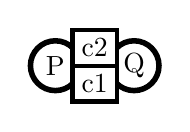
\begin{tikzpicture}[node distance   = 4 cm]
      \GraphInit[vstyle=Normal]
      \tikzset{LabelStyle/.style = {draw}}
      \SetVertexNormal[Shape = circle,
                       TextColor = black,
                       LineWidth = 2pt]
      \Vertex{P}
      \EA(P){Q}
      \SetUpEdge[style={->,bend right,ultra thick},labelstyle = {draw}]
      \Edge[label=c1](P)(Q)
      \Edge[label=c2](Q)(P)
    \end{tikzpicture}
  \end{center}
  \caption{What to do when two opposite PRI ALT meet?}
  \label{prialt}
\end{figure}

We haven't implemented {\it PRI ALT}\cite{occam}, even though it's implemented
in all the other libraries we compare ours to. The primary reason is that it's
not described in the Occam reference manual what will happend if two {\it PRI
ALT} met, see figure \ref{prialt}. On the other hand we also don't implement
{\it FAIR SELECT} because it's not really implemented in Occam and both the
versions from JCSP and C++CSP2 differs from each other but both agree on that
over time as our implementation, will ensure, statistically, that all the
process will be called the same amount of time and no process can be
indefinitely starved.

Because we don't have implemented {\it PRI ALT}, this also affects that it will
not give sense to implemented {\it SKIP GUARDS}. {\it SKIP GUARDS} are only
usefull whenever you have the guarded process as the final process in the list.
Because we use randomness, we could encounter this guarded process before
another guarded process that was ready to read/write. Following this we also
don't have the possibility to implement {\it polling}, again based on the
randomness of alternation in CSP (external choice).

About the implementation of {\it TIME GUARDS} we could achieve this by creating
a guarded process, put the thread to sleep the desired amount of time, then wake
up and send the message. Because this is possible, we leave up to the developer
responsability to do it himself.

The \emph{read} and \emph{write} functions are semantically equivalent to a select that has exactly 
one guard.

The semantics of the select so far is to block until one of the guards become ready. The obvious
way to define a select with no guards at all is therefore to block indefinatly, causing a deadlock.
Preferably, the thread would not take up any further resources in this case (since it's trivial to 
detect), and thus we attempt to terminate the thread by throwing an exception. If stack traces are
enabled, and the empty select is an error, this might also provide the programmer with more information
to determine where the error occured.

In JCSP and C++CSP2 you can provide a list of flags that specify if a guard is
active or inactive. We do not provide this as it is just as easy to simply
filter the list of guarded processes.

\subsection{Termination of process networks}
Since few applications run forever, termination of process networks should be
considered.

Another way to implement this is to send a special termination message. However,
that requires insertion of termination logic for every communication where the
process might receive a termination message. Additionally, if the readers want
to terminate the writers of a channel, it will often require a dedicated channel
just for termination messages.

If there are multiple processes that listen on a channel, it would also be hard
to ensure that they had all received the termination message before the process
sending it shuts down. To keep track of this you might need to know the number
of processes that are listening or are going to listen on the channel, which
might not even be possible to determine. The process that wants to send the
terminating process could loop forever, repeating the termination message to
anybody who read from the channel, but then that process could never shut down.

In PyCSP, JCSP and C++CSP2, a channel may be \emph{poisoned}. Once a channel
has been poisoned, reading from or writing to that channel causes an exception.
The exception may be handled, thus allowing the process to clean up, propagate
the poison, or even ignore the poisoning. That way, the process remains in
control of it's own lifespan. A channel that has been poisoned can never become
unpoisoned. We provide the same construct:

\begin{verbatim}
Csp.poison c 
\end{verbatim}

Read and write guards become ready if their channel is poisoned, and an
alternation may thus chose to throw a PoisonException if one or more of its
guards' channels are poisoned.

In order to shut down process networks, which may have intrnal subnetworks, it
is nessecary to propagate the poison to the other processes in the network. As
mentioned, this can be done in the handler for PoisonException. PyCSP
automatically poisons channels that are arguments to process constructors. In 
the following PyCSP example:
\begin{verbatim}
def foo(in,out):
    while True:
        x = in()
        out(x)
        
        poisonChannel(in)
\end{verbatim}
Even if we only poison the input channel, as soon as we try to read again on
the input channel then we get poisoned and throw a poison exception. By doing
this we then iterate through the parameters in the constructor checking if
they are channels, if they are we poison. In our example we have the {\it in}
and {\it out}, both get poisoned and hereby we have propagated the poison
received by the input channel. For more information on this, look at
\cite{pycsp}.

In many cases this is the desired behaviour. JCSP and C++CSP2 do not provide it,
and neither do we due to technical issues (see section \ref{implementation}).

\subsection{Permissions}

PyCSP, JCSP and C++CSP2 provide a concept called \emph{channel ends}, which are
handles to channels though which you can only read or only write (or some other
set of permissions). This is useful for specifying what a process might do with
a channel, so unintended use of a channel can be caught early.

We provide this through a set of functions, each of which takes a channel
returns a handle with only a specific set of permissions:

\begin{verbatim}
let i = Csp.read_only c
\end{verbatim}

It is a compile time error to attempt to write to or poison the returned handle.
The permissions are provided purely through the type system, and none of the
functions can add permissions. See secion \ref{implementation} for the complete
set.

\section{Implementation}
\missing{
- Mention that we do everything within OCaml's type system.\\
- Mention why we can't have parallelism.\\
- Mention why it isn't interesting to use system threads.\\
- Describe why we cannot provide automatic poison propagation.\\
}
\label{implementation}


\subsection{Channels and alternation}
A one-to-one channel is a channel that only allows one procees to read from it
and one process 
to write to it. It may be implemented as a state machine as shown in figure \ref{channel-state}.
When the channel is in the NobodyWaiting state and a process tries to read from the channel,
it enters the ReaderWaiting state. When a writer comes along and tries to write to a channel
in this state, it returns to the NobodyWaiting state, transfers the message, and only then
allows the two processes to continue. The WriterWaiting state works in much the same way.

\begin{figure}[h]
\centering
    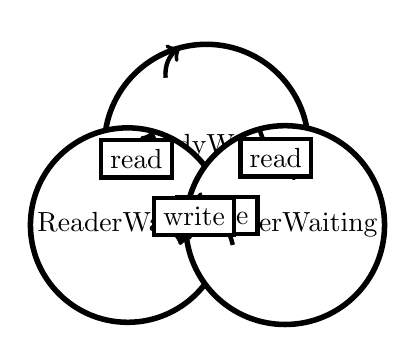
\begin{tikzpicture}[node distance   = 5 cm]
      \GraphInit[vstyle=Normal]
      \tikzset{LabelStyle/.style =   {draw}}
      \SetVertexNormal[TextColor = white,
                       LineColor = white]
      \Vertex{Start}
      \SetVertexNormal[Shape = circle,
                       TextColor = black,
                       LineWidth = 2pt]
      \SOEA(Start){NobodyWaiting}
      \SOWE(NobodyWaiting){ReaderWaiting}
      \SOEA(NobodyWaiting){WritterWaiting}
      \SetUpEdge[style={->,bend right,ultra thick},labelstyle = {draw}]
      \Edge[label=read](NobodyWaiting)(ReaderWaiting)
      \Edge[label=write](NobodyWaiting)(WritterWaiting)
      \SetUpEdge[style={->,bend right,ultra thick},labelstyle = {draw}]
      \Edge[label=write](ReaderWaiting)(NobodyWaiting)
      \Edge[label=read](WritterWaiting)(NobodyWaiting)
      \SetUpEdge[style={->,bend left,ultra thick}]
      \Edge(Start)(NobodyWaiting)
    \end{tikzpicture}
\caption{Simplified channel state (poison and multi-read/write not shown)}
\label{channel-state}
\end{figure}

From any state, the channel might be poisoned and enter the Poisoned state. If it was in the
ReaderWaiting or the WriterWaiting state, the waiting process will wake up and throw a special
exception. Any further attempts to read from or write to the channel will result in this 
exception being thrown again.

Any-to-any channels places no restrictions on the number of processes that can
read from or write to it. To implement these we extend the above to keep a queue
of readers (when in the ReaderWaiting state) or writers (when in the
WriterWaiting state).

The choice of using a queue gives a stronger guarentee than CSP gives, namely that no processes
will be starved. By starvation we mean to say that a process waiting to read or write on the
channel can be blocked indefinately even though an infinite number of messages is transmitted
over the channel. This would happen with a stack if another process is always ready to read or 
write again before the channel was ready to accomodate the starving process. The starving process
would always be put behind the eager process with a stack, but with a queue, the starving process
will always advance in the queue every time a message is transmitted, guarenteeing that it will
eventually get it's turn.

\goodbreak
The internal state for channels looks like this:

\begin{verbatim}
type 'a channel_state
    = NobodyWaiting 
    | ReaderWaiting of (Condition.t * ('a -> unit)) list
    | WriterWaiting of (Condition.t * (unit -> 'a)) list
    | Poisoned
\end{verbatim}

Both readers and writers have a condition variable that they are waiting on
while in the queue. Readers have a function that when given a value may perform
a side effect $(\alpha \to unit)$, and writers have a function that may perform
a side effect and then returns the value to be written. These functions are
only supposed to be called when transmitting a value. The side effects in both
cases is to change the internal state of the waiting process and to remove it
from all the channels it is waiting on. The state change is such that the
process can tell that the transmit has happened, thus allowing it to continue.
In the case of the readers, it stores the value transmitted.

A process registers itself for reading or writing on any number of channels via
the select construct, which takes a list of guarded processes. It augments each
with a condition variable unique to the process. Then shuffles the list in order
to avoid starvation as discussed in section \ref{api-design}. It checks if any
of the channels associated with the guarded processes are poisoned, and if
that is the case, throws a PoisonException. This is done by calling
\emph{check\_poison} for each of them, which is part of the following record:

\begin{verbatim}
type 'a concrete_guard = {
    attempt: unit -> (unit -> 'a) option;
    check_poison: unit -> bool;
    subscribe: ('a concrete_guard) list -> 
        ((unit -> 'a) option) ref -> unit;
    unsubscribe: unit -> unit;
}
\end{verbatim}

Otherwise it calls \emph{attempt} on each of them until one succeeds.
When \emph{attempt} succeeds, it carries out a transmission and returns $Some\
f$ where $f$ is a function that when called carries out the process part of the
guarded process and returns its result. Otherwise it returns $None$. If any of
them succeeds, $f$ is applied (to unit) and the result is returned.

If none of the attempts succeed, it \emph{subscribes} each guarded process.
This means creating a function that fits into the channel waiting queue
as discussed earlier, and putting it into the queue. Then it enters a loop
where it waits on the process' condition variable each iteration. When woken up
due to a signal on the condition variable, it checks if it has been involved in
a transmission, and then executes the process part of the chosen guarded
process.

We use a lock that is global to the library in order to protect the state
associated with channels and processes from concurrent mutation (and
thus race conditions). This lock is only taken when first trying to read from a
channel, or right after a process has been woken up. We claim that this won't
lead to performance degradation, since OCaml's threads only provides concurrency
though time-sharing \cite{ocaml-threads}. The execution of the process part of
guarded processes are done outside this lock since they do not require it and
because they may run for a very long time (or even diverge).

Read and write are implemented as selects a trivial guarded process:
\begin{verbatim}
let read c = select [read_guard c (fun x -> x)]
let write c v = select [write_guard c v (fun () -> ())]
\end{verbatim}

\missing{
- How do you get rid of this lock? (useful for porting). It is hard because you don't know which
channels you will touch before you have chosen a target process to transmit to/from. If you knew
that, you could simply take their locks in some well defined order (thus avoiding deadlock). \\
}

\subsection{Alternation}

\begin{verbatim}
type ('a, 'b) channel = ('a channel_state) ref
\end{verbatim}

The phantom type 'b is used for the channel permissions. This is enforced solely via the type
system, and is represented with a product of three booleans values: read * write * poison.
Reading, writing and poisoning are initially enabled for a channel, but handles with less 
permissions can be obtained through the functions shown in figure \ref{channel-permissions}. 
Permissions can only be taken away, not gained, which is evident from the types of the 
functions, for example: 

\begin{verbatim}
val read_poison_only : ('a, on * _ * on) channel -> 
                       ('a, on * off * on) channel
\end{verbatim}

Apart from the type, all of these functions are simply identity functions. We provide a
type alias \texttt{'a t = ('a, on * on * on) channel} for people who don't want to write the
longer (often optional) type annotations that the permission types incur.

\begin{figure}[h]
\centering
\begin{tabular}{c|c|c|l}
Read & Write & Poison & Function \\
\hline
0 & 0 & 0 & (useless) \\
0 & 0 & 1 & poison\_only \\
0 & 1 & 0 & write\_only \\
0 & 1 & 1 & write\_poison\_only \\
1 & 0 & 0 & read\_only \\
1 & 0 & 1 & read\_poison\_only \\
1 & 1 & 0 & read\_write\_only \\
1 & 1 & 1 & (default) \\
\end{tabular}
\caption{Channel permissions}
\label{channel-permissions}
\end{figure}

\subsection{Processes}

\section{Test, performance and examples}
\label{testexamples}
One of the goals for this project was that we needed to implement a simple
network on top of the API, Fibonacci, and a more complex one but because Ocaml
doesn't have support for parallelism, as mentioned in the section \ref{apidesign},
we decided to make a Webproxy, with a build in cache so we show that we actually
use overlapping I/O.

But before we made this two applications we needed to know the limitations of
Ocamls thread library and I/O library.

A detailed description on how to run the test can be seen in appendix
\ref{appendixOcamltest}.

\subsection{Ocaml tests}
\label{ocamltests}
\begin{table}[!h]
  \begin{center}
    \begin{tabular}{|p{3cm}|p{8.5cm}|c|}
      \hline
      File name &
      Description &
      Result \\
      \hline
      maxthreads.ml (user thread) &
      The application creates as many threads as possible, once it reaches
      about 15.000 it stops spawning more threads.&
      OK \\
      \hline
      maxthreads.ml (system thread) &
      The application creates as many threads as possible, once it reaches
      about 100 it stops spawning more threads.&
      OK \\
      \hline
      nonblocking.ml &
      We run to processes in parallel. The first process whats for user input
      and the second process after a seconds delay reads the first line from
      the its own source code file and writes the line to stdout.&
      OK \\
      \hline
    \end{tabular} 
    \caption{The test checks Ocaml implementation of the threadlibrary and I/O.}
    \label{testtable}
  \end{center}
\end{table}

\subsubsection{Maxthreads}
In this test we try to find an upperbound of how many threads we can create,
user threads and/or system threads. In the first case when using user threads we
find that after creating between 15.000 - 20.000 threads the application
freezes. We are not able to find any kind of documentation that can helps us
verify that it's a deadlock or a maximum number of threads allowed for an
application to create. If we run the test several times, we will see that
each application will be able to create about those 15.000 - 20.000 threads.

In the second test based on maxthreads, we use system threads and as before
the application freezes but just after creating about 100 threads.

Even though we didn't find any kind of documentation on the maximum number
of threads to create, if we read read the documentation for the thread library
we can see that {\it Thread.create} terminates when the {\it func args}
returns either normally or by rasing an uncaught exception. In this last case
the exception will be printed to the standard error but not be propagated to
the parent thread. Because we don't see any kind of message we must assume
that the created threads are still running in the background until we join
them and if we joined them, we will suspend the calling thread until the
child thread was terminated, which will be never cos we run them forever with:
\begin{verbatim}
let loop () = while true do () done
\end{verbatim}

\subsubsection{Nonblocking}
To implement the Webproxy we need to know if one of the processes is waiting
to recieve a chunck of data, if it block the IO until it has recieved the data
or if another process that is also waiting for a chunck.

We discovered that Ocaml support non-blocking IO so it will be no problem have
several clients waiting to recieve data from our Webproxy. An example could
be a client that connects over the Webproxy to a very slow website. The website
can only deliver a small amount of data every second. If another client that
also connects over the Webproxy to a fast website. While the first client
waits to recieve data from the webserver, the second client can read chunks
of data from the fast website.

So what we have done is that we run two processes in parallel, the first one
waits for the user input, while the second one reads a line from it's own
code file after a second of waiting (Thread.sleep). As we can see in the test
the second process is able to read the line even if the first process waits,
hereby we can see that we don't have non-blocking I/O.

\subsection{OcamlCSP tests}
\label{ocamlcsptests}
\subsubsection{Channel permisions}
One of the features this API has is that you have the possibility to set 
read/write/poision permissions on the channels. With this test we will
demostrate where this is useful. What we do is that we have to components
that just counts integers. When the second counter reaches $20$ we want
to poison the whole network. But we have sat the first count to only count
to 10 and it will shutdown the hole network through the {\it stop}
component from the {\it Legoland} library. But this is a problem, we don't
want the first counter to shut down the network so we add {\it write\_only}
to counter components output channel. This will result in a compiler error
because the {\it stop} component once it's poisoned it propagates the poison
to all the other channels, but we have just defined our output channel to
only allow write.

We now make a {\it custom\_stop} component which only propagates poison to
the input channel. We are now able to compile and run the application knowing
that our first counter will never shutdown our network through poison.

Even though we don't allow to propagate poison whenever the second counter
reaches it's number and poison the printer component. Then when the first
counter will write over the {\it custom\_stop} component, it will actually
raise a {\it PoisonException} which will be progated back to the counter
ensuring that all of the processes terminate and hereby ensuring that network
shuts down correctly.

\subsubsection{Alternation}
Based on the same code file as the one used to permision, we added a small
{\it guard} test which read from the two counters components whenever one of
them are ready. By setting the first counter to only send 5 numbers, we can
actually check that when setting the second counter to the double we can see
that the {\it custom\_printer} component will see if any of the to
{\it read\_guards} are ready to read from the counters and because one stop
early it will keep reading from the second.

Both results can be seen in appendix \ref{appendixOcamlcsptest}.

\subsection{Performance}
\label{performance}
Even though we don't set focus on performance and optimization, we still wanted
to implement the Commstime\cite{vinterpycsp} process that's used to compare
PyCSP against JCSP.

\subsubsection{Commstime}
The only change we made to the code is that we use {\it Unix.gettimeofday} in
order to get the same time precision as Pythons {\it time.time} has. By running
both application on the same computer\footnote{Macbook Pro 2,6 GHz Core 2 Duo
4GB RAM. Mac OS 10.5.7}, we achieve a execution time that it's about twenty
times faster. Results can be seen in appendix \ref{appendixPerformance}.

\subsection{Examples}
\label{examples}

\subsubsection{Fibonacci}
\begin{figure}[h]
  \begin{center}
    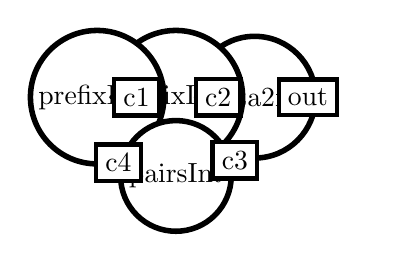
\begin{tikzpicture}[node distance   = 4 cm]
      \GraphInit[vstyle=Normal]
      \tikzset{LabelStyle/.style =   {draw}}
      \SetVertexNormal[TextColor = white,
                       LineColor = white]
      \Vertex{Out}
      \SetVertexNormal[Shape = circle,
                       TextColor = black,
                       LineWidth = 2pt]
      \WE(Out){delta2int}
      \WE(delta2int){prefixInt0}
      \WE(prefixInt0){prefixInt1}
      \SO(prefixInt0){pairsInt}
      \SetUpEdge[style={->,ultra thick},labelstyle = {draw}]
      \Edge[label=out](delta2int)(Out)
      \Edge[label=c2](prefixInt0)(delta2int)
      \Edge[label=c1](prefixInt1)(prefixInt0)
      \SetUpEdge[style={->,bend left,ultra thick},labelstyle = {draw}]
      \Edge[label=c3](delta2int)(pairsInt)
      \Edge[label=c4](pairsInt)(prefixInt1)
    \end{tikzpicture}
  \end{center}
  \caption{FibonacciInt, a CSP component from the Legoland Library.}
  \label{fibonaccicomp}
\end{figure}

This test, once we have implemented all the {\it Legoland}\cite{vintercsp}
components, was a very easy and straight forward task. Even though that it
looks like this network doesn't do much it was very useful to discover that
our first implementation didn't work correctly.

\begin{figure}[h]
  \begin{center}
    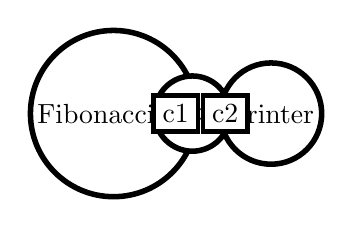
\begin{tikzpicture}[node distance   = 4 cm]
      \GraphInit[vstyle=Normal]
      \tikzset{LabelStyle/.style = {draw}}
      \SetVertexNormal[Shape = circle,
                       TextColor = black,
                       LineWidth = 2pt]
      \Vertex{FibonacciInt}
      \EA(FibonacciInt){Stop}
      \EA(Stop){Printer}
      \SetUpEdge[style={->,ultra thick},labelstyle = {draw}]
      \Edge[label=c1](FibonacciInt)(Stop)
      \Edge[label=c2](Stop)(Printer)
    \end{tikzpicture}
  \end{center}
  \caption{Fibonacci CSP network with stop component.}
  \label{fibonacci}
\end{figure}

Another thing was that we implemented our {\it Legoland} components as
recursive function, but not tail-recursive, after running this application
for a lot of iteration, about 75.000, we began to get messages of stack
overflow. Once we rewrote the components from recursive to using {\it while true
do} we was able to run more than a 1.000.000 iterations, We supouse we can
run even more but we didn't test it out.

A description on how this simple network works can be seen in figure
\ref{fibonaccicomp} and \ref{fibonacci} where we use the {\it Legoland
fibonacciInt} component running in parallel with a {\it stop} component which,
ensures that the network shuts down correctly after the number of iterations
given as the first parameter, and a {\it printer} component which prints out to
the screen the Fibonacci numbers.

Other examples on how to write some simple processes and them put them together
running in parallel in another process can be seen in our {\it CSP component 
library (Legoland)}, see  {\it appendix \ref{appendixLegoland}}.

\subsubsection{Webproxy}
\begin{figure}[h]
  \begin{center}
    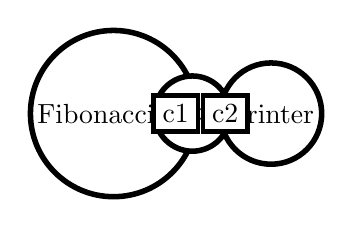
\begin{tikzpicture}[node distance = 4 cm]
      \GraphInit[vstyle=Normal]
      \tikzset{LabelStyle/.style =   {draw}}
      \SetVertexNormal[Shape = circle,
                       TextColor = black,
                       LineWidth = 2pt]
      \Vertex{FibonacciInt}
      \EA(FibonacciInt){Stop}
      \EA(Stop){Printer}
      \SetUpEdge[style={->,ultra thick},labelstyle = {draw}]
      \Edge[label=c1](FibonacciInt)(Stop)
      \Edge[label=c2](Stop)(Printer)
    \end{tikzpicture}
  \end{center}
  \caption{Webproxy CSP network.}
  \label{webproxy}
\end{figure}

TODO: this is critical (refactoring of code? it's almost impossible to draw
the network diagram) ...

\section{Conclusion}
\label{conclusion}

TODO: Write the conclusion last ...

%If we compare how Brian Vinter teaches CSP\cite{vintercsp}:
%\begin{center}
%\begin{verbatim}
%PairsInt (in, out) = Delta2Int (in, a, c) || 
%                     TailInt (a, b) || 
%                     PlusInt (b, c, out) 
%\end{verbatim}
%\end{center}

%versus how we implement the simple network:

%\begin{verbatim}
%let pairsInt i o () =
%  let a = Csp.new_channel () in
%  let b = Csp.new_channel () in
%  let c = Csp.new_channel () in
%    Csp.parallel [
%      delta2int i a c;
%      tailint a b;
%      plusint b c o;
%    ]
%\end{verbatim}

%We can see that there is almost no difference beside the {\it parallel operator}
%and definition of the channel variables.

% ----------------------------------------------------------------------
% Bibliography
% ----------------------------------------------------------------------
\newpage
\begin{thebibliography}{99}

\bibitem[Ocaml]{ocaml}
:\\
Objective Caml\\
Xavier Leroy, Jérôme Vouillon, Damien Doligez, Didier Rémy\\
National Institute for Research in Computer and Control Sciences\\
http://caml.inria.fr/ocaml/\\
Last visited: $24^{th}$ july 2009

\bibitem[Hoare 04]{hoare}
:\\
Communicating Sequential Processes\\
C. A. R. Hoare\\
Prentice Hall International; (June 24, 2004)\\
ISBN-10: 0-13-153271-5\\
ISBN-13: 978-0-13-153271-7\\
http://www.usingcsp.com/cspbook.pdf

\bibitem[PyCSP]{pycsp}
:\\
PyCSP - Communicating Sequential Processes for Python\\
John Markus Bjørndalen, Brian Vinter and Otto Anshus\\
Department of Computer Science, University of Tromsø and\\
Department of Computer Science, University of Copenhagen\\
http://www.cs.uit.no/$\sim$johnm/publications/pdf/bjorndalen2007pycsp.pdf\\
Last visited: $26^{th}$ july 2009

\bibitem[JCSP]{jcsp}
:\\
Communicating Sequential Processes for Java\texttrademark (JCSP)\\
Peter Welch and Paul Austin\\
University of Kent at Canterbury\\
http://www.cs.kent.ac.uk/projects/ofa/jcsp/\\
Last visited: $26^{th}$ july 2009

\bibitem[C++CSP2]{cppcsp2}
:\\
C++CSP2: A Many-to-Many Threading Model for Multicore Architectures\\
Brown,  Neil C. C.\\
University of Kent at Canterbury\\
ISBN-13: 978-1586037673\\
http://www.cs.kent.ac.uk/projects/ofa/c++csp/\\
Last visited: $26^{th}$ july 2009

\newpage
\bibitem[Occam]{occam}
:\\
Occam 2 Reference Manual\\
C. A. R. Hoare\\
Prentice Hall; (May 1988)\\
ISBN-10: 0136293123\\
ISBN-13: 978-0136293125

\bibitem[Vinter, PyCSP]{vinterpycsp}
:\\
PyCSP. The beginning of a CSP library for Python\\
Brian Vinter\\
Department of Computer Science. University of Copenhagen\\
http://isis.ku.dk/kurser/blob.aspx?feltid=224718\\
Last visited: $20^{th}$ july 2009

\bibitem[Vinter, CSP]{vintercsp}
:\\
Threading\\
Brian Vinter\\
Department of Computer Science. University of Copenhagen\\
http://isis.ku.dk/kurser/blob.aspx?feltid=224185\\
Last visited: $20^{th}$ july 2009

\end{thebibliography}
% ----------------------------------------------------------------------

\appendix
\newpage
\secttoc
\section{Appendix: Source code}
\label{appendixSrc}

\scriptsize
\subsection{API}
\label{appendixAPI}
\includecode{csp.mli}{../source/csp.mli}
\includecode{csp.ml}{../source/csp.ml}
\subsection{A CSP Utility Library}
\label{appendixCspu}
\includecode{cspu.ml}{../source/cspu.ml}
\subsection{A CSP Component Library (Legoland)}
\label{appendixLegoland}
\includecode{legoland.ml}{../source/legoland.ml}


\newpage
\section{Appendix: Documentation}
\label{appendixDoc}
The documentation can be created with following command:

\runtest{ocamldoc -html -d ../docs/ csp.mli}
\begin{center}
  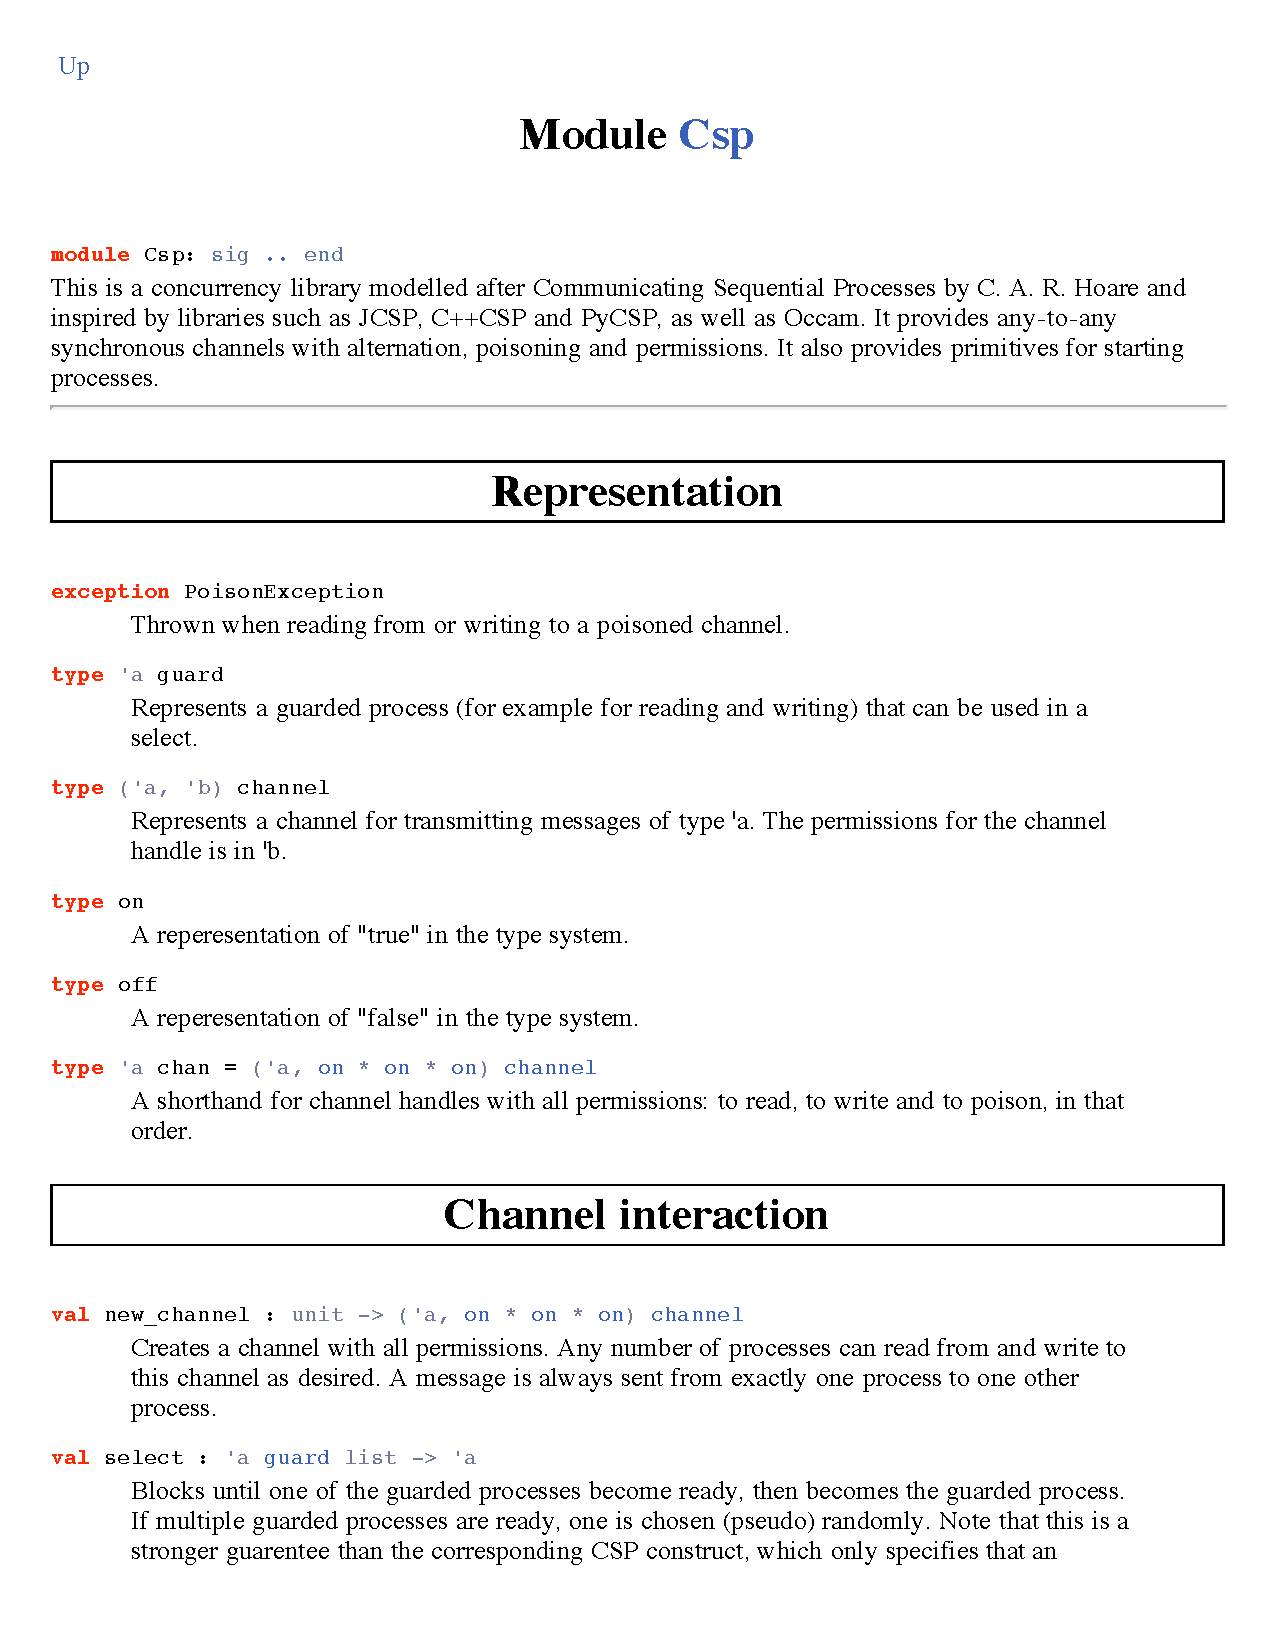
\includepdf[pages=-]{../docs/csp.pdf}
\end{center}

\newpage
\secttoc
\section{Appendix: Test, performance and examples}
\label{appendixTest}

\subsection{Ocaml tests}
\label{appendixOcamltest}
\subsubsection{Maxthreads}
\includecode{maxthreads.ml}{../test/maxthreads.ml}
\runtest{ocamlc -vmthread unix.cma threads.cma maxthreads.ml -o maxthreads \&\&
  ./maxthreads}
\includeoutput{userMaxThreads.txt}{test/userMaxThreads.txt}
\runtest{ocamlc -thread unix.cma threads.cma maxthreads.ml -o maxthreads \&\&
  ./maxthreads}
\includeoutput{sysMaxThreads.txt}{test/sysMaxThreads.txt}

\subsubsection{Nonblocking}
\includecode{nonblocking.ml}{../test/nonblocking.ml}
\runtest{ocamlc -vmthread threads.cma unix.cma nonblocking.ml -o nonblocking
  \&\& ./nonblocking}
\includeoutput{nonblocking.txt}{test/nonblocking.txt}

\subsection{OcamlCSP tests}
\label{appendixOcamlcsptest}
\subsubsection{Channel permisions}
\includecode{permission.ml}{../test/permission.ml}
\runtest{./buildPermission.sh \&\& ./buildPermission}
\includeoutput{permision\_error.txt}{test/permision_error.txt}

\subsubsection{Alternation}
\includeoutput{alternation\_one\_guard.txt}{test/alternation_one_guard.txt}
\includeoutput{alternation\_poison.txt}{test/alternation_poison.txt}

\subsection{Performance}
\label{appendixPerformance}
\subsubsection{Commstime}
\includecode{commstime.ml}{../test/commstime.ml}
\runtest{./buildCommstime.sh \&\& ./commstime}
\includeoutput{ocamlcsp\_commstime.txt}{test/ocamlcsp_commstime.txt}
\includeoutput{pycsp\_commstime.txt}{test/pycsp_commstime.txt}

\subsection{Examples}
\subsubsection{Fibonacci}
\includecode{fibCSP.ml}{../test/fibCSP.ml}
\runtest{./buildFibCSP.sh \&\& ./buildFibCSP}
\includeoutput{fibonacci.txt}{test/fibonacci.txt}

\newpage
\subsubsection{Webproxy}
\includecode{proxyCSP.ml}{../test/proxyCSP.ml}
\includecode{server.rb}{../test/web/server.rb}
Start two sequential webservers (ruby):

\runtest{ruby server.rb 4040 0.1 \&}

\runtest{ruby server.rb 4041 0.3 \&}


Start the webproxy:

\runtest{./buildProxy.sh \&\& ./proxyCSP \&}


Add the webproxy to the terminal session:

\runtest{export http\_proxy=http://localhost:8080}


Retrieve the file foo.mp3 from the first webserver:

\runtest{wget http://localhost:4040/foo.mp3}
\includeoutput{proxy\_get\_file\_first\_time.txt}{
  test/proxy_get_file_first_time.txt}


Retrieve the file foo.mp3 again from the first webserver (cache):

\runtest{wget http://localhost:4040/foo.mp3}

\includeoutput{proxy\_get\_file\_second\_time.txt}{
  test/proxy_get_file_second_time.txt}


Retrieve concurrent the files bar.mp3 and foo.mp3 from the two webservers:

\includeoutput{proxy\_same\_time\_bar.txt}{
  test/proxy_same_time_bar.txt}
\includeoutput{proxy\_same\_time\_foo.txt}{
  test/proxy_same_time_foo.txt}

\newpage
\section{Appendix: Other}
\subsection{Why systhreads? (Xavier Leroy)}
\label{appendixSysthreads}
{\tt
  \scriptsize
  \input{appendix/whySysthreads.txt}
  \normalsize
}

\end{document}
